\chapter{Preliminaries}
\label{chapter:preliminaries}

In order to be able to explain the solution approach we have to declare to, which programs are considered within the Geometric Nontermination. Furthermore we have to define a few structures we work on.

\section{Non-Termination}
The definition of non-termination is the most essential considering a technique proving it. Non-termination can be defined as a specific input to a program $p$, such that $p$ runs in an infinite loop.
Proving termination is much harder than proving non-termination, since we only have to determine one case, which fit's the condition of running into an infinite loop. \newline
Non-termination is obviously still undecidable, since otherwise the halting problem would be decidable, nevertheless there are a large variety of possibilities to prove non-termination as we will see in this paper.

\section{Integer Term Rewrite System(\its)}
\label{sec:its}
In order to apply the upcoming procedure we have to define what structure the approach works on. The derivation of an \its from source code is described in \autoref{sec:aprove}. Considering the following approach we will look at a \its in a more superficial way. The composition of a \its considered in this paper is shown in \autoref{fig:its-structure}.\newline
\begin{figure}[H]
	\begin{lstlisting}[escapechar=!]
		!$\overbrace{f_x}^{(1)} \qquad\qquad \rightarrow \overbrace{f_y}^{(2)} (v_1, \dots v_n) :|: cond_1$!
		!$f_y(\underbrace{v_1, \dots v_n}_{(3)}) \>\> \rightarrow \>\> f_y \>(\underbrace{v^\prime_1,\dots v^\prime_n}_{(3)})  :|: \underbrace{cond_2}_{(4)}$!
	\end{lstlisting}
	\caption{The structure of a \its considered in this paper.}
	\label{fig:its-structure}
\end{figure}
%QUESTION: Explanation in text or in figure?

The considered program shown in \autoref{fig:its-structure} consists of a set of structure elements necessary to be defined:
\begin{enumerate}[leftmargin=1]
	\item[(1)] A function symbol consisting of no variables is a \textit{start function symbol} and is the first symbol to use. Further explanation in (line 1) and \autoref{fig:structure-example-TRS}.
	\item[(2)] A function symbol denoting a current program-state
	\item[(3)] The variables of a function symbol denoting the change of the variables by applying the term rewriting rule. The value of $v^\prime_i$ is a linear update of the variables $v_j$ $1 \le j \le n$ in \stdLinInt. \footnote{The \stdLinInt has the following pattern: $ a_1*v_1 + \dots + a_n*v_n + c$, where $a_i , v_i, c \in \mathbb{Z}$, $1 \le i\le n$. 
		Also it is important that $a_i * v_i$ has this order and not $v_i*a_i$} 
	\item[(4)] The conditional term of the form $\text{(in)equation}_1 \text{ \&\& } \dots \text{ \&\& } \text{(in)equation}_m$ $m \in \mathbb{N}$, where $\text{(in)equation}_i$ contains only $v_j$ $1 \le j \le n$ defined further in \autoref{sec:derivation-guard}.
	\item[(line 1)] The first line is the rewriting rule the program starts with and can be seen as a declaration of initial values of some variables. An example is shown in \autoref{fig:structure-example-TRS}
	\item[(line 2)] Such a rule is a self-looping rule considered within this approach to define further computations. Other looping rules will be presented in \autoref{sec:structure-improvement}.
\end{enumerate} 

In general a \its can have rules of other forms, like $f_x(v_1, \dots v_n) \rightarrow f_y(v^\prime_1, \dots v^\prime_k) :|: cond$ where $n \ne k$ can occur, but these rules are for now not considered.

\section{Geometric Nontermination Argument (GNA)}
Adapted from Jan Leikes and Matthias Heizmanns paper \textit{Geometric Nontermination Arguments} \cite{leike2014geometric} I will define the considered programs, define the \stem and \loopt and finally state the definition of Geometric Nontermination Arguments.

\subsection{Considered Programs}
The considered programs in the Geometric Nontermination are not bound to a special programming language. The paper works on so called Linear-Lasso Programs, which in fact are also used within \aprove to derive the so called (int-)TRS, stated in \autoref{sec:aprove}. Because of the also stated conversion of the language into a \seg and further analysis the applicability of \gna's are not bound to any programming language. \newline
In order to define the specific conditions under which we can use the approach, we take the language \tool{Java} as an example.
\subsection{Structure}
\label{sec:structure}
The structure of the considered programs is quite simple. They contain an optional declaration of the used variables and a \code{while}-loop. Even though \tool{Java} would not accept this the conversion to \tool{llvm} would still be sound. An example of a fulfilling \tool{Java} program is shown in \autoref{fig:structure-example-java}. 
\begin{itemize}
	\item The \stem: \newline
		The initialization and optional declaration of variables used within the \code{while}-loop. In the example line 3 and 4 are considered the \stem. Also only $b$ is declared.
	\item The guard: \newline
		The guard of the \code{while}-loop is essential to restrict $a$  as we will see in \autoref{sec:stem-var}. With the restriction of $a+b\ge 4 $ we can prove termination for $a < 3$ without further analysis, and also to prove termination assume that $a \ge 3$.
	\item The linear Updates: \newline
		The updates of the variables within the \code{while}-loop are the most essential part for termination, since their value determine if the guard still holds. The approach works with only linear updates of the variables, so for every variable $v_i$ where $1\le i\le n$ we can have a $v_i=a_1*v_1+...+a_n*v_n$ with $n \in \mathbb{N}$. Note since we work on int-TRS it is sufficient for $a_i$ to be in $\mathbb{Z}$. 	
\end{itemize} 

\begin{figure}[h]
	\begin{lstlisting}[language = java, escapechar = !, linewidth=0.6\linewidth]
	int main(){
		
		int a;!\tikz[remember picture] \node [] (a) {};!
		int b=1;!\tikz[remember picture] \node [] (b) {};!
		
		while(a+b>=4){! \tikz[remember picture] \node [] (c) {}; !
			a=3*a+b;!\tikz[remember picture] \node [] (d) {}; !
			b=2*b;!\tikz[remember picture] \node [] (e) {}; !
		}
	}		
	\end{lstlisting}
	\begin{tikzpicture}[remember picture, overlay, 
		every edge/.append style = {dashedarrow},
		every node/.append style = {explNode},
	text width = 2.5cm ]
		\node[above right = .2cm and 3.1 cm of a] (A) {the \textit{STEM}};
		\draw[rounded corners=5pt] (A.west) edge (a.east);
		\draw (A.west) edge (b.east);
		
		\node[below = of A, right = of c] (B) {the guard};
		\draw (B.west) edge (c.east);
		
		\node[right = 4cm of d, below = of B] (C) {the linear update};
		\draw (C.west) edge (d.east);
		\draw (C.west) edge (e.east);
	\end{tikzpicture}
%	\lstinputlisting{src/listings/preliminaries-consideredPrograms-example-java.java}		
	\caption{A \tool{Java} program fulfilling the conditions to be applicable}
	\label{fig:structure-example-java}
\end{figure}
The guard and linear updates together form the so called \loopt. 

Through the in \autoref{sec:its} described procedure and given structure we receive the to \autoref{fig:structure-example-java} equivalent \its shown in \autoref{fig:structure-example-TRS}. As we can see the original program can be recognized quite easily. The first rule in line 1 denotes the \stem, while the second line equals the loop \loopt.

\begin{figure}[H]
	\begin{lstlisting}[linewidth=1.4\textwidth, escapechar = !]
!$\overbrace{f_1	     \rightarrow f_2(1+3*c,2)   :|: c>2 \text{ \&\& } 8<3*c}^{\text{\stem}}$!
!$\underbrace{\underbrace{f_2(a,b) \rightarrow f_2(3*a+b,2*b)}_{\text{linear update}} :|: \underbrace{3*a>29 \text{ \&\& } a+b>11 \text{ \&\& } 31<3*a+b \text{ \&\& } 3<2*b}_{\text{guards}}}_{\text{\loopt}}$!
	\end{lstlisting}
	\caption{The \its corresponding to the \tool{Java} program in \autoref{fig:structure-example-java}}
	\label{fig:structure-example-TRS}
\end{figure}
 Neglecting the conditional terms for now the declaration of $b$ is set in line 1 obviously to 2, because of the one circle the \seg has to compute in order to find a loop. The definition of $a$ is more difficult and will be shown within REF \autoref{sec:stem}. 
Also the update within line 2 is the same as in \autoref{fig:structure-example-java} line 7 and 8. \newline

\subsection{Necessary Definitions}
In order to be able to define the key element of this approach, the \gna, we have to define a number of matrices and constant vectors, which are used to derive such a \gna. 

\begin{definition}[\stem]
	The \stem is denoted as a vector $x \in \mathbb{Z}^n$, where $n$ is the number of variables within the rule of the start function symbols right hand side of a \its. The values of $x$ can be constants or defined by conditions. Examples are shown within \autoref{sec:stem}.
\end{definition}

\begin{definition}[Guard Matrix, Guard Constants]
	\label{def:guard}
	Let $n \in \mathbb{N}$ be the number of distinct variables, $v_i$ $1 \le i \le n$ the $i$-th distinct variable name , $m \in \mathbb{N}$ be the number of guards, $r_i$ $1 \le i \le m$ the $i$-th guard, $a_{i,j} \in \mathbb{Z}$ $1\le i \le n$, $1 \le j \le m$ the factor of $v_i$ in $g_j$ and $c_i \in \mathbb{Z}$ be the constant term within $r_j$. \newline
		
	Then the \guardmatrix $G \in \mathbb{Z}^{m\times n}$ is defined as $G_{i,j}=a_{i,j} $ and \guardconstants $g \in \mathbb{Z}^m$ are defined as $g_i = c_i$.
\end{definition}
\begin{example}
	The corresponding \guardmatrix to \autoref{fig:structure-example-TRS} is $G = \begin{pmatrix} 3 & 0 \\ 1 & 1 \\ 3 & 1 \\ 0 & 2 \end{pmatrix}$ and the \guardconstants is $g= \begin{pmatrix} 29 \\ 11 \\ 31 \\ 3 \end{pmatrix}$
\end{example}

\begin{definition}[Update Matrix, Update Constants]
	\label{def:update}
	Let $n \in \mathbb{N}$ be the number of distinct variables, $v_i$ $1 \le i \le n$ the $i$-th distinct		variable name, $m \in \mathbb{N}$ the arity of the function symbol of the right hand side, $m_i$ $1 \le i \le m$ the $i$-th variable definition of the right hand sight's function symbol, $a_{i,j} \in \mathbb{Z}$ $1 \le i \le n$ $1 \le j \le m$ be the factor of variable $v_i$ in variable definition $m_i$ and $c_i \in \mathbb{Z}$ $1 \le i \le m$ the constant term of $m_i$. \newline
	
	Then the \updatematrix $U \in \mathbb{Z}^{m \times n}$ is defined as $U_{i,j}=a_{i,j}$ and \updateconstants $u \in \mathbb{Z}^m$ are defined as $g_i = c_i$.
\end{definition}
\begin{example}
	The corresponding \updatematrix to \autoref{fig:structure-example-TRS} is $U = \begin{pmatrix} 3 & 1 \\ 0 & 2 \end{pmatrix}$ and the \updateconstants are $u = \begin{pmatrix} 0 \\ 0 \end{pmatrix}$.
\end{example}

\begin{definition}[Iteration Matrix, Iteration Constants]
	\label{def:iteration}
	Let $G$ be the \guardmatrix, $g$ the \guardconstants, $U$ the \updatematrix, $u$ the \updateconstants, $n\in \mathbb{N}$ the number of variables and $m \in \mathbb{N}$ the number of conditional terms. \newline
	Also let \textbf{0} be a matrix of the size of $G$ with only entry's 0 and $I$ denote the identity matrix with the size of $U$. \newline
	
	The \iterationmatrix $A \in \mathbb{Z}^{2*n+m \times 2*n}$, which defines one complete execution of the \loopt, and the \iterationconstants $b\in \mathbb{Z}^{2*n+m} $ is defined as
	\begin{figure}[H]
		\centering
		$A = \begin{pmatrix} G & \textbf{0} \\ M & -I \\ -M & I \end{pmatrix}$ and $b = \begin{pmatrix} g \\ -u \\ u \end{pmatrix}$ \cite{leike2014geometric}
	\end{figure}	
\end{definition}

\begin{definition}[LOOP]
	The \loopt is defined as a tuple $(A, b)$, where $A$ is the \iterationmatrix and $b$ the \iterationconstants of an \its. (See: \autoref{sec:loop})
\end{definition}

Now we can define the key element, which was originally defined for \tool{linear lasso programs}. 

\begin{definition}[Geometric Non Termination Argument]
	\label{def:gna}
	A tuple of the form:
	\begin{figure}[H]
		\centering
		$(x, y_1, \dots, y_k, \lambda_1, \dots, \lambda_k, \mu_1, \dots, \mu_{k-1})$
	\end{figure}  
	\vspace{-1em}
	is called a \gna for a program = $(\stem, \loopt)$ with $n$ variables iff all of the following statements hold:
	\begin{itemize}
		\setlength{\itemindent}{1in}
		\item[(domain)] $x, y_1, \dots, y_k \in \mathbb{R}^n$, $\lambda_1, \dots \lambda_k, \mu_1, \dots \mu_{k-1} \ge 0$
		\item[(init)] x represents the \startterm (\stem)
		\item[(point)] $A\begin{pmatrix} x \\ x + \sum_i y_i \end{pmatrix} \le b$
		\item[(ray)] $A\begin{pmatrix} y_i \\ \lambda_i y_i + \mu_{i-1} y_{i-1} \end{pmatrix} \le 0$ for all $1 \le i \le k$
	\end{itemize}
	Note that $y_0 = \mu_0 = 0$ is set for the ray instead of a case distinction. \cite{leike2014geometric}
\end{definition}

The usage of such a \gna is justified by the following sentence:
\begin{satz}
	\label{sen:gna-nonterm}
	If a \gna $a$ for a program $p$ exists, then $p$ does not terminate. \cite{leike2014geometric} 
\end{satz}

\section{Reverse-Polish-Notation-Tree}
\label{sec:rpntree}
Within the program of deriving a \gna it happens that we get a mathematical term in the so-called \textit{Polish Notation} or \textit{Reverse Polish Notation in prefix notation}, which is a special form of rewriting a, in our case linear, expression to compute the solution efficiently using a stack. Within our program we use this kind of notation to parse it into our own tree-structure to do further analysis. \cite{wikirpn}

As shown in \autoref{dia:RPN-classdiagram} we have an \code{abstract} root, subclasses for every occurring type of element within the \its, a \code{static} parsing of a given term and an exception for parsing exceptions.
An example for the \rpntree is shown in \autoref{ex:rpntree}

\begin{figure}[H]
	\centering	
	% Graphic for TeX using PGF
% Title: D:\Dokumente\GitHub\Bachelorarbeit\Arbeitstagebuch\src\04.07.2017-RPNTree-classdiagram.dia
% Creator: Dia v0.97.2
% CreationDate: Wed Aug 30 19:22:10 2017
% For: Timo Bergerbusch
% \usepackage{tikz}
% The following commands are not supported in PSTricks at present
% We define them conditionally, so when they are implemented,
% this pgf file will use them.
\ifx\du\undefined
  \newlength{\du}
\fi
\setlength{\du}{15\unitlength}
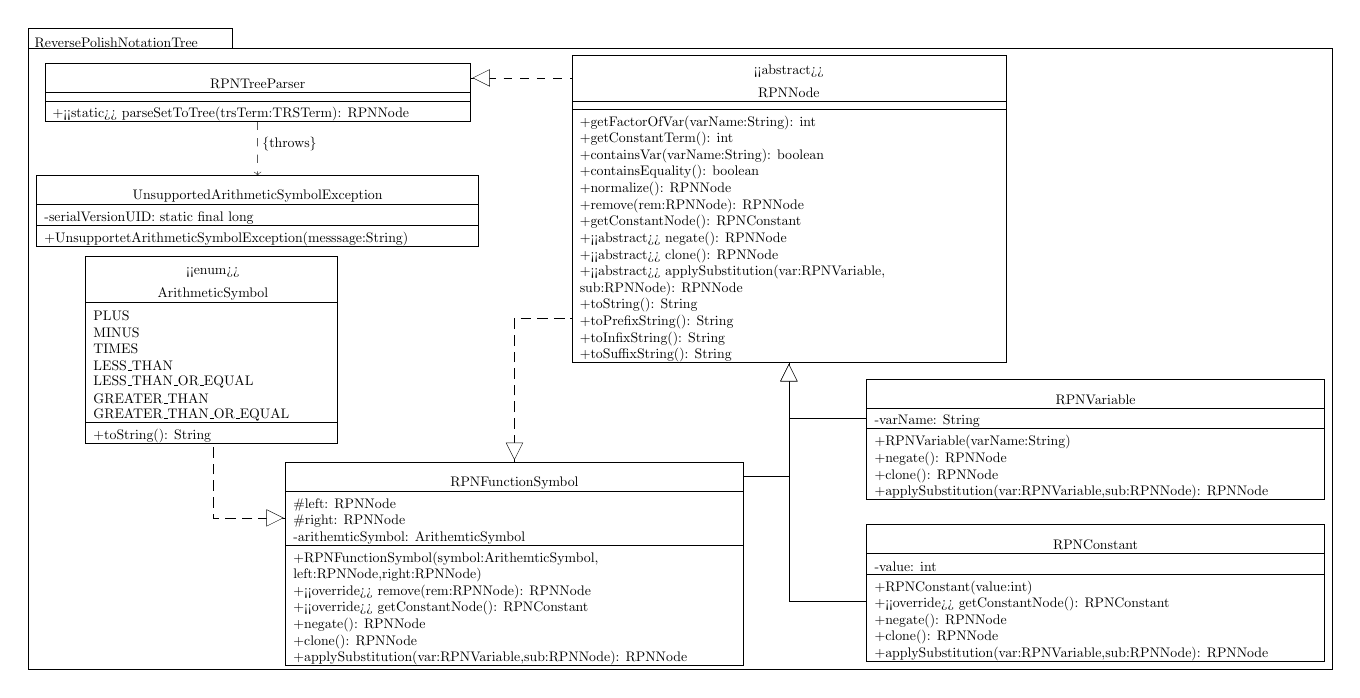
\begin{tikzpicture}[scale=0.5, every node/.style={scale=0.5}]
\pgftransformxscale{1.000000}
\pgftransformyscale{-1.000000}
\definecolor{dialinecolor}{rgb}{0.000000, 0.000000, 0.000000}
\pgfsetstrokecolor{dialinecolor}
\definecolor{dialinecolor}{rgb}{1.000000, 1.000000, 1.000000}
\pgfsetfillcolor{dialinecolor}
\pgfsetlinewidth{0.010000\du}
\pgfsetdash{}{0pt}
\definecolor{dialinecolor}{rgb}{1.000000, 1.000000, 1.000000}
\pgfsetfillcolor{dialinecolor}
\fill (-2.412990\du,34.090900\du)--(-2.412990\du,64.000000\du)--(60.422652\du,64.000000\du)--(60.422652\du,34.090900\du)--cycle;
\definecolor{dialinecolor}{rgb}{0.000000, 0.000000, 0.000000}
\pgfsetstrokecolor{dialinecolor}
\draw (-2.412990\du,34.090900\du)--(-2.412990\du,64.000000\du)--(60.422652\du,64.000000\du)--(60.422652\du,34.090900\du)--cycle;
\definecolor{dialinecolor}{rgb}{1.000000, 1.000000, 1.000000}
\pgfsetfillcolor{dialinecolor}
\fill (-2.412990\du,33.090900\du)--(-2.412990\du,34.090900\du)--(7.412010\du,34.090900\du)--(7.412010\du,33.090900\du)--cycle;
\definecolor{dialinecolor}{rgb}{0.000000, 0.000000, 0.000000}
\pgfsetstrokecolor{dialinecolor}
\draw (-2.412990\du,33.090900\du)--(-2.412990\du,34.090900\du)--(7.412010\du,34.090900\du)--(7.412010\du,33.090900\du)--cycle;
% setfont left to latex
\definecolor{dialinecolor}{rgb}{0.000000, 0.000000, 0.000000}
\pgfsetstrokecolor{dialinecolor}
\node[anchor=west] at (-2.312990\du,33.790900\du){ReversePolishNotationTree};
\pgfsetlinewidth{0.010000\du}
\pgfsetdash{}{0pt}
\definecolor{dialinecolor}{rgb}{1.000000, 1.000000, 1.000000}
\pgfsetfillcolor{dialinecolor}
\fill (23.800000\du,34.400000\du)--(23.800000\du,36.600000\du)--(44.705000\du,36.600000\du)--(44.705000\du,34.400000\du)--cycle;
\definecolor{dialinecolor}{rgb}{0.000000, 0.000000, 0.000000}
\pgfsetstrokecolor{dialinecolor}
\draw (23.800000\du,34.400000\du)--(23.800000\du,36.600000\du)--(44.705000\du,36.600000\du)--(44.705000\du,34.400000\du)--cycle;
% setfont left to latex
\definecolor{dialinecolor}{rgb}{0.000000, 0.000000, 0.000000}
\pgfsetstrokecolor{dialinecolor}
\node at (34.252500\du,35.160000\du){<<abstract>>};
% setfont left to latex
\definecolor{dialinecolor}{rgb}{0.000000, 0.000000, 0.000000}
\pgfsetstrokecolor{dialinecolor}
\node at (34.252500\du,36.200000\du){RPNNode};
\definecolor{dialinecolor}{rgb}{1.000000, 1.000000, 1.000000}
\pgfsetfillcolor{dialinecolor}
\fill (23.800000\du,36.600000\du)--(23.800000\du,37.000000\du)--(44.705000\du,37.000000\du)--(44.705000\du,36.600000\du)--cycle;
\definecolor{dialinecolor}{rgb}{0.000000, 0.000000, 0.000000}
\pgfsetstrokecolor{dialinecolor}
\draw (23.800000\du,36.600000\du)--(23.800000\du,37.000000\du)--(44.705000\du,37.000000\du)--(44.705000\du,36.600000\du)--cycle;
\definecolor{dialinecolor}{rgb}{1.000000, 1.000000, 1.000000}
\pgfsetfillcolor{dialinecolor}
\fill (23.800000\du,37.000000\du)--(23.800000\du,49.200000\du)--(44.705000\du,49.200000\du)--(44.705000\du,37.000000\du)--cycle;
\definecolor{dialinecolor}{rgb}{0.000000, 0.000000, 0.000000}
\pgfsetstrokecolor{dialinecolor}
\draw (23.800000\du,37.000000\du)--(23.800000\du,49.200000\du)--(44.705000\du,49.200000\du)--(44.705000\du,37.000000\du)--cycle;
% setfont left to latex
\definecolor{dialinecolor}{rgb}{0.000000, 0.000000, 0.000000}
\pgfsetstrokecolor{dialinecolor}
\node[anchor=west] at (23.950000\du,37.660000\du){+getFactorOfVar(varName:String): int};
% setfont left to latex
\definecolor{dialinecolor}{rgb}{0.000000, 0.000000, 0.000000}
\pgfsetstrokecolor{dialinecolor}
\node[anchor=west] at (23.950000\du,38.460000\du){+getConstantTerm(): int};
% setfont left to latex
\definecolor{dialinecolor}{rgb}{0.000000, 0.000000, 0.000000}
\pgfsetstrokecolor{dialinecolor}
\node[anchor=west] at (23.950000\du,39.260000\du){+containsVar(varName:String): boolean};
% setfont left to latex
\definecolor{dialinecolor}{rgb}{0.000000, 0.000000, 0.000000}
\pgfsetstrokecolor{dialinecolor}
\node[anchor=west] at (23.950000\du,40.060000\du){+containsEquality(): boolean};
% setfont left to latex
\definecolor{dialinecolor}{rgb}{0.000000, 0.000000, 0.000000}
\pgfsetstrokecolor{dialinecolor}
\node[anchor=west] at (23.950000\du,40.860000\du){+normalize(): RPNNode};
% setfont left to latex
\definecolor{dialinecolor}{rgb}{0.000000, 0.000000, 0.000000}
\pgfsetstrokecolor{dialinecolor}
\node[anchor=west] at (23.950000\du,41.660000\du){+remove(rem:RPNNode): RPNNode};
% setfont left to latex
\definecolor{dialinecolor}{rgb}{0.000000, 0.000000, 0.000000}
\pgfsetstrokecolor{dialinecolor}
\node[anchor=west] at (23.950000\du,42.460000\du){+getConstantNode(): RPNConstant};
% setfont left to latex
\definecolor{dialinecolor}{rgb}{0.000000, 0.000000, 0.000000}
\pgfsetstrokecolor{dialinecolor}
\node[anchor=west] at (23.950000\du,43.260000\du){+<<abstract>> negate(): RPNNode};
% setfont left to latex
\definecolor{dialinecolor}{rgb}{0.000000, 0.000000, 0.000000}
\pgfsetstrokecolor{dialinecolor}
\node[anchor=west] at (23.950000\du,44.060000\du){+<<abstract>> clone(): RPNNode};
% setfont left to latex
\definecolor{dialinecolor}{rgb}{0.000000, 0.000000, 0.000000}
\pgfsetstrokecolor{dialinecolor}
\node[anchor=west] at (23.950000\du,44.860000\du){+<<abstract>> applySubstitution(var:RPNVariable,};
\definecolor{dialinecolor}{rgb}{0.000000, 0.000000, 0.000000}
\pgfsetstrokecolor{dialinecolor}
\node[anchor=west] at (23.950000\du,45.660000\du){                                sub:RPNNode): RPNNode};
% setfont left to latex
\definecolor{dialinecolor}{rgb}{0.000000, 0.000000, 0.000000}
\pgfsetstrokecolor{dialinecolor}
\node[anchor=west] at (23.950000\du,46.460000\du){+toString(): String};
% setfont left to latex
\definecolor{dialinecolor}{rgb}{0.000000, 0.000000, 0.000000}
\pgfsetstrokecolor{dialinecolor}
\node[anchor=west] at (23.950000\du,47.260000\du){+toPrefixString(): String};
% setfont left to latex
\definecolor{dialinecolor}{rgb}{0.000000, 0.000000, 0.000000}
\pgfsetstrokecolor{dialinecolor}
\node[anchor=west] at (23.950000\du,48.060000\du){+toInfixString(): String};
% setfont left to latex
\definecolor{dialinecolor}{rgb}{0.000000, 0.000000, 0.000000}
\pgfsetstrokecolor{dialinecolor}
\node[anchor=west] at (23.950000\du,48.860000\du){+toSuffixString(): String};
\pgfsetlinewidth{0.010000\du}
\pgfsetdash{}{0pt}
\definecolor{dialinecolor}{rgb}{1.000000, 1.000000, 1.000000}
\pgfsetfillcolor{dialinecolor}
\fill (38.000000\du,50.000000\du)--(38.000000\du,51.400000\du)--(60.060000\du,51.400000\du)--(60.060000\du,50.000000\du)--cycle;
\definecolor{dialinecolor}{rgb}{0.000000, 0.000000, 0.000000}
\pgfsetstrokecolor{dialinecolor}
\draw (38.000000\du,50.000000\du)--(38.000000\du,51.400000\du)--(60.060000\du,51.400000\du)--(60.060000\du,50.000000\du)--cycle;
% setfont left to latex
\definecolor{dialinecolor}{rgb}{0.000000, 0.000000, 0.000000}
\pgfsetstrokecolor{dialinecolor}
\node at (49.030000\du,51.000000\du){RPNVariable};
\definecolor{dialinecolor}{rgb}{1.000000, 1.000000, 1.000000}
\pgfsetfillcolor{dialinecolor}
\fill (38.000000\du,51.400000\du)--(38.000000\du,52.400000\du)--(60.060000\du,52.400000\du)--(60.060000\du,51.400000\du)--cycle;
\definecolor{dialinecolor}{rgb}{0.000000, 0.000000, 0.000000}
\pgfsetstrokecolor{dialinecolor}
\draw (38.000000\du,51.400000\du)--(38.000000\du,52.400000\du)--(60.060000\du,52.400000\du)--(60.060000\du,51.400000\du)--cycle;
% setfont left to latex
\definecolor{dialinecolor}{rgb}{0.000000, 0.000000, 0.000000}
\pgfsetstrokecolor{dialinecolor}
\node[anchor=west] at (38.150000\du,52.060000\du){-varName: String};
\definecolor{dialinecolor}{rgb}{1.000000, 1.000000, 1.000000}
\pgfsetfillcolor{dialinecolor}
\fill (38.000000\du,52.400000\du)--(38.000000\du,55.800000\du)--(60.060000\du,55.800000\du)--(60.060000\du,52.400000\du)--cycle;
\definecolor{dialinecolor}{rgb}{0.000000, 0.000000, 0.000000}
\pgfsetstrokecolor{dialinecolor}
\draw (38.000000\du,52.400000\du)--(38.000000\du,55.800000\du)--(60.060000\du,55.800000\du)--(60.060000\du,52.400000\du)--cycle;
% setfont left to latex
\definecolor{dialinecolor}{rgb}{0.000000, 0.000000, 0.000000}
\pgfsetstrokecolor{dialinecolor}
\node[anchor=west] at (38.150000\du,53.060000\du){+RPNVariable(varName:String)};
% setfont left to latex
\definecolor{dialinecolor}{rgb}{0.000000, 0.000000, 0.000000}
\pgfsetstrokecolor{dialinecolor}
\node[anchor=west] at (38.150000\du,53.860000\du){+negate(): RPNNode};
% setfont left to latex
\definecolor{dialinecolor}{rgb}{0.000000, 0.000000, 0.000000}
\pgfsetstrokecolor{dialinecolor}
\node[anchor=west] at (38.150000\du,54.660000\du){+clone(): RPNNode};
% setfont left to latex
\definecolor{dialinecolor}{rgb}{0.000000, 0.000000, 0.000000}
\pgfsetstrokecolor{dialinecolor}
\node[anchor=west] at (38.150000\du,55.460000\du){+applySubstitution(var:RPNVariable,sub:RPNNode): RPNNode};
\pgfsetlinewidth{0.010000\du}
\pgfsetdash{}{0pt}
\definecolor{dialinecolor}{rgb}{1.000000, 1.000000, 1.000000}
\pgfsetfillcolor{dialinecolor}
\fill (38.000000\du,57.000000\du)--(38.000000\du,58.400000\du)--(60.060000\du,58.400000\du)--(60.060000\du,57.000000\du)--cycle;
\definecolor{dialinecolor}{rgb}{0.000000, 0.000000, 0.000000}
\pgfsetstrokecolor{dialinecolor}
\draw (38.000000\du,57.000000\du)--(38.000000\du,58.400000\du)--(60.060000\du,58.400000\du)--(60.060000\du,57.000000\du)--cycle;
% setfont left to latex
\definecolor{dialinecolor}{rgb}{0.000000, 0.000000, 0.000000}
\pgfsetstrokecolor{dialinecolor}
\node at (49.030000\du,58.000000\du){RPNConstant};
\definecolor{dialinecolor}{rgb}{1.000000, 1.000000, 1.000000}
\pgfsetfillcolor{dialinecolor}
\fill (38.000000\du,58.400000\du)--(38.000000\du,59.400000\du)--(60.060000\du,59.400000\du)--(60.060000\du,58.400000\du)--cycle;
\definecolor{dialinecolor}{rgb}{0.000000, 0.000000, 0.000000}
\pgfsetstrokecolor{dialinecolor}
\draw (38.000000\du,58.400000\du)--(38.000000\du,59.400000\du)--(60.060000\du,59.400000\du)--(60.060000\du,58.400000\du)--cycle;
% setfont left to latex
\definecolor{dialinecolor}{rgb}{0.000000, 0.000000, 0.000000}
\pgfsetstrokecolor{dialinecolor}
\node[anchor=west] at (38.150000\du,59.060000\du){-value: int};
\definecolor{dialinecolor}{rgb}{1.000000, 1.000000, 1.000000}
\pgfsetfillcolor{dialinecolor}
\fill (38.000000\du,59.400000\du)--(38.000000\du,63.600000\du)--(60.060000\du,63.600000\du)--(60.060000\du,59.400000\du)--cycle;
\definecolor{dialinecolor}{rgb}{0.000000, 0.000000, 0.000000}
\pgfsetstrokecolor{dialinecolor}
\draw (38.000000\du,59.400000\du)--(38.000000\du,63.600000\du)--(60.060000\du,63.600000\du)--(60.060000\du,59.400000\du)--cycle;
% setfont left to latex
\definecolor{dialinecolor}{rgb}{0.000000, 0.000000, 0.000000}
\pgfsetstrokecolor{dialinecolor}
\node[anchor=west] at (38.150000\du,60.060000\du){+RPNConstant(value:int)};
% setfont left to latex
\definecolor{dialinecolor}{rgb}{0.000000, 0.000000, 0.000000}
\pgfsetstrokecolor{dialinecolor}
\node[anchor=west] at (38.150000\du,60.860000\du){+<<override>> getConstantNode(): RPNConstant};
% setfont left to latex
\definecolor{dialinecolor}{rgb}{0.000000, 0.000000, 0.000000}
\pgfsetstrokecolor{dialinecolor}
\node[anchor=west] at (38.150000\du,61.660000\du){+negate(): RPNNode};
% setfont left to latex
\definecolor{dialinecolor}{rgb}{0.000000, 0.000000, 0.000000}
\pgfsetstrokecolor{dialinecolor}
\node[anchor=west] at (38.150000\du,62.460000\du){+clone(): RPNNode};
% setfont left to latex
\definecolor{dialinecolor}{rgb}{0.000000, 0.000000, 0.000000}
\pgfsetstrokecolor{dialinecolor}
\node[anchor=west] at (38.150000\du,63.260000\du){+applySubstitution(var:RPNVariable,sub:RPNNode): RPNNode};
\pgfsetlinewidth{0.010000\du}
\pgfsetdash{}{0pt}
\definecolor{dialinecolor}{rgb}{1.000000, 1.000000, 1.000000}
\pgfsetfillcolor{dialinecolor}
\fill (10.000000\du,54.000000\du)--(10.000000\du,55.400000\du)--(32.060000\du,55.400000\du)--(32.060000\du,54.000000\du)--cycle;
\definecolor{dialinecolor}{rgb}{0.000000, 0.000000, 0.000000}
\pgfsetstrokecolor{dialinecolor}
\draw (10.000000\du,54.000000\du)--(10.000000\du,55.400000\du)--(32.060000\du,55.400000\du)--(32.060000\du,54.000000\du)--cycle;
% setfont left to latex
\definecolor{dialinecolor}{rgb}{0.000000, 0.000000, 0.000000}
\pgfsetstrokecolor{dialinecolor}
\node at (21.030000\du,55.000000\du){RPNFunctionSymbol};
\definecolor{dialinecolor}{rgb}{1.000000, 1.000000, 1.000000}
\pgfsetfillcolor{dialinecolor}
\fill (10.000000\du,55.400000\du)--(10.000000\du,58.000000\du)--(32.060000\du,58.000000\du)--(32.060000\du,55.400000\du)--cycle;
\definecolor{dialinecolor}{rgb}{0.000000, 0.000000, 0.000000}
\pgfsetstrokecolor{dialinecolor}
\draw (10.000000\du,55.400000\du)--(10.000000\du,58.000000\du)--(32.060000\du,58.000000\du)--(32.060000\du,55.400000\du)--cycle;
% setfont left to latex
\definecolor{dialinecolor}{rgb}{0.000000, 0.000000, 0.000000}
\pgfsetstrokecolor{dialinecolor}
\node[anchor=west] at (10.150000\du,56.060000\du){\#left: RPNNode};
% setfont left to latex
\definecolor{dialinecolor}{rgb}{0.000000, 0.000000, 0.000000}
\pgfsetstrokecolor{dialinecolor}
\node[anchor=west] at (10.150000\du,56.860000\du){\#right: RPNNode};
% setfont left to latex
\definecolor{dialinecolor}{rgb}{0.000000, 0.000000, 0.000000}
\pgfsetstrokecolor{dialinecolor}
\node[anchor=west] at (10.150000\du,57.660000\du){-arithemticSymbol: ArithemticSymbol};
\definecolor{dialinecolor}{rgb}{1.000000, 1.000000, 1.000000}
\pgfsetfillcolor{dialinecolor}
\fill (10.000000\du,58.000000\du)--(10.000000\du,63.800000\du)--(32.060000\du,63.800000\du)--(32.060000\du,58.000000\du)--cycle;
\definecolor{dialinecolor}{rgb}{0.000000, 0.000000, 0.000000}
\pgfsetstrokecolor{dialinecolor}
\draw (10.000000\du,58.000000\du)--(10.000000\du,63.800000\du)--(32.060000\du,63.800000\du)--(32.060000\du,58.000000\du)--cycle;
% setfont left to latex
\definecolor{dialinecolor}{rgb}{0.000000, 0.000000, 0.000000}
\pgfsetstrokecolor{dialinecolor}
\node[anchor=west] at (10.150000\du,58.660000\du){+RPNFunctionSymbol(symbol:ArithemticSymbol,};
\definecolor{dialinecolor}{rgb}{0.000000, 0.000000, 0.000000}
\pgfsetstrokecolor{dialinecolor}
\node[anchor=west] at (10.150000\du,59.460000\du){                   left:RPNNode,right:RPNNode)};
% setfont left to latex
\definecolor{dialinecolor}{rgb}{0.000000, 0.000000, 0.000000}
\pgfsetstrokecolor{dialinecolor}
\node[anchor=west] at (10.150000\du,60.260000\du){+<<override>> remove(rem:RPNNode): RPNNode};
% setfont left to latex
\definecolor{dialinecolor}{rgb}{0.000000, 0.000000, 0.000000}
\pgfsetstrokecolor{dialinecolor}
\node[anchor=west] at (10.150000\du,61.060000\du){+<<override>> getConstantNode(): RPNConstant};
% setfont left to latex
\definecolor{dialinecolor}{rgb}{0.000000, 0.000000, 0.000000}
\pgfsetstrokecolor{dialinecolor}
\node[anchor=west] at (10.150000\du,61.860000\du){+negate(): RPNNode};
% setfont left to latex
\definecolor{dialinecolor}{rgb}{0.000000, 0.000000, 0.000000}
\pgfsetstrokecolor{dialinecolor}
\node[anchor=west] at (10.150000\du,62.660000\du){+clone(): RPNNode};
% setfont left to latex
\definecolor{dialinecolor}{rgb}{0.000000, 0.000000, 0.000000}
\pgfsetstrokecolor{dialinecolor}
\node[anchor=west] at (10.150000\du,63.460000\du){+applySubstitution(var:RPNVariable,sub:RPNNode): RPNNode};
\pgfsetlinewidth{0.010000\du}
\pgfsetdash{}{0pt}
\pgfsetmiterjoin
\pgfsetbuttcap
{
\definecolor{dialinecolor}{rgb}{0.000000, 0.000000, 0.000000}
\pgfsetfillcolor{dialinecolor}
% was here!!!
\definecolor{dialinecolor}{rgb}{0.000000, 0.000000, 0.000000}
\pgfsetstrokecolor{dialinecolor}
\draw (34.252500\du,49.200000\du)--(34.252500\du,51.900000\du)--(38.000000\du,51.900000\du);
}
\definecolor{dialinecolor}{rgb}{0.000000, 0.000000, 0.000000}
\pgfsetstrokecolor{dialinecolor}
\draw (34.252500\du,50.111803\du)--(34.252500\du,51.900000\du)--(38.000000\du,51.900000\du);
\pgfsetmiterjoin
\definecolor{dialinecolor}{rgb}{1.000000, 1.000000, 1.000000}
\pgfsetfillcolor{dialinecolor}
\fill (34.652500\du,50.111803\du)--(34.252500\du,49.311803\du)--(33.852500\du,50.111803\du)--cycle;
\pgfsetlinewidth{0.010000\du}
\pgfsetdash{}{0pt}
\pgfsetmiterjoin
\definecolor{dialinecolor}{rgb}{0.000000, 0.000000, 0.000000}
\pgfsetstrokecolor{dialinecolor}
\draw (34.652500\du,50.111803\du)--(34.252500\du,49.311803\du)--(33.852500\du,50.111803\du)--cycle;
% setfont left to latex
\pgfsetlinewidth{0.010000\du}
\pgfsetdash{}{0pt}
\pgfsetmiterjoin
\pgfsetbuttcap
{
\definecolor{dialinecolor}{rgb}{0.000000, 0.000000, 0.000000}
\pgfsetfillcolor{dialinecolor}
% was here!!!
\definecolor{dialinecolor}{rgb}{0.000000, 0.000000, 0.000000}
\pgfsetstrokecolor{dialinecolor}
\draw (34.252500\du,49.200000\du)--(34.252500\du,60.700000\du)--(38.000000\du,60.700000\du);
}
\definecolor{dialinecolor}{rgb}{0.000000, 0.000000, 0.000000}
\pgfsetstrokecolor{dialinecolor}
\draw (34.252500\du,50.111803\du)--(34.252500\du,60.700000\du)--(38.000000\du,60.700000\du);
\pgfsetmiterjoin
\definecolor{dialinecolor}{rgb}{1.000000, 1.000000, 1.000000}
\pgfsetfillcolor{dialinecolor}
\fill (34.652500\du,50.111803\du)--(34.252500\du,49.311803\du)--(33.852500\du,50.111803\du)--cycle;
\pgfsetlinewidth{0.010000\du}
\pgfsetdash{}{0pt}
\pgfsetmiterjoin
\definecolor{dialinecolor}{rgb}{0.000000, 0.000000, 0.000000}
\pgfsetstrokecolor{dialinecolor}
\draw (34.652500\du,50.111803\du)--(34.252500\du,49.311803\du)--(33.852500\du,50.111803\du)--cycle;
% setfont left to latex
\pgfsetlinewidth{0.010000\du}
\pgfsetdash{}{0pt}
\pgfsetmiterjoin
\pgfsetbuttcap
{
\definecolor{dialinecolor}{rgb}{0.000000, 0.000000, 0.000000}
\pgfsetfillcolor{dialinecolor}
% was here!!!
\definecolor{dialinecolor}{rgb}{0.000000, 0.000000, 0.000000}
\pgfsetstrokecolor{dialinecolor}
\draw (34.252500\du,49.200000\du)--(34.252500\du,54.700000\du)--(32.060000\du,54.700000\du);
}
\definecolor{dialinecolor}{rgb}{0.000000, 0.000000, 0.000000}
\pgfsetstrokecolor{dialinecolor}
\draw (34.252500\du,50.111803\du)--(34.252500\du,54.700000\du)--(32.060000\du,54.700000\du);
\pgfsetmiterjoin
\definecolor{dialinecolor}{rgb}{1.000000, 1.000000, 1.000000}
\pgfsetfillcolor{dialinecolor}
\fill (34.652500\du,50.111803\du)--(34.252500\du,49.311803\du)--(33.852500\du,50.111803\du)--cycle;
\pgfsetlinewidth{0.010000\du}
\pgfsetdash{}{0pt}
\pgfsetmiterjoin
\definecolor{dialinecolor}{rgb}{0.000000, 0.000000, 0.000000}
\pgfsetstrokecolor{dialinecolor}
\draw (34.652500\du,50.111803\du)--(34.252500\du,49.311803\du)--(33.852500\du,50.111803\du)--cycle;
% setfont left to latex
\pgfsetlinewidth{0.010000\du}
\pgfsetdash{}{0pt}
\definecolor{dialinecolor}{rgb}{1.000000, 1.000000, 1.000000}
\pgfsetfillcolor{dialinecolor}
\fill (0.369629\du,44.098102\du)--(0.369629\du,46.298102\du)--(12.5\du,46.298102\du)--(12.5\du,44.098102\du)--cycle;
\definecolor{dialinecolor}{rgb}{0.000000, 0.000000, 0.000000}
\pgfsetstrokecolor{dialinecolor}
\draw (0.369629\du,44.098102\du)--(0.369629\du,46.298102\du)--(12.5\du,46.298102\du)--(12.5\du,44.098102\du)--cycle;
% setfont left to latex
\definecolor{dialinecolor}{rgb}{0.000000, 0.000000, 0.000000}
\pgfsetstrokecolor{dialinecolor}
\node at (6.5\du,44.858102\du){<<enum>>};
% setfont left to latex
\definecolor{dialinecolor}{rgb}{0.000000, 0.000000, 0.000000}
\pgfsetstrokecolor{dialinecolor}
\node at (6.5\du,45.898102\du){ArithmeticSymbol};
\definecolor{dialinecolor}{rgb}{1.000000, 1.000000, 1.000000}
\pgfsetfillcolor{dialinecolor}
\fill (0.369629\du,46.298102\du)--(0.369629\du,52.098102\du)--(12.5\du,52.098102\du)--(12.5\du,46.298102\du)--cycle;
\definecolor{dialinecolor}{rgb}{0.000000, 0.000000, 0.000000}
\pgfsetstrokecolor{dialinecolor}
\draw (0.369629\du,46.298102\du)--(0.369629\du,52.098102\du)--(12.5\du,52.098102\du)--(12.5\du,46.298102\du)--cycle;
% setfont left to latex
\definecolor{dialinecolor}{rgb}{0.000000, 0.000000, 0.000000}
\pgfsetstrokecolor{dialinecolor}
\node[anchor=west] at (0.519629\du,46.958102\du){ PLUS};
% setfont left to latex
\definecolor{dialinecolor}{rgb}{0.000000, 0.000000, 0.000000}
\pgfsetstrokecolor{dialinecolor}
\node[anchor=west] at (0.519629\du,47.758102\du){ MINUS};
% setfont left to latex
\definecolor{dialinecolor}{rgb}{0.000000, 0.000000, 0.000000}
\pgfsetstrokecolor{dialinecolor}
\node[anchor=west] at (0.519629\du,48.558102\du){ TIMES};
% setfont left to latex
\definecolor{dialinecolor}{rgb}{0.000000, 0.000000, 0.000000}
\pgfsetstrokecolor{dialinecolor}
\node[anchor=west] at (0.519629\du,49.358102\du){ LESS\_THAN};
% setfont left to latex
\definecolor{dialinecolor}{rgb}{0.000000, 0.000000, 0.000000}
\pgfsetstrokecolor{dialinecolor}
\node[anchor=west] at (0.519629\du,50.158102\du){ LESS\_THAN\_OR\_EQUAL};
% setfont left to latex
\definecolor{dialinecolor}{rgb}{0.000000, 0.000000, 0.000000}
\pgfsetstrokecolor{dialinecolor}
\node[anchor=west] at (0.519629\du,50.958102\du){ GREATER\_THAN};
% setfont left to latex
\definecolor{dialinecolor}{rgb}{0.000000, 0.000000, 0.000000}
\pgfsetstrokecolor{dialinecolor}
\node[anchor=west] at (0.519629\du,51.758102\du){ GREATER\_THAN\_OR\_EQUAL};
\definecolor{dialinecolor}{rgb}{1.000000, 1.000000, 1.000000}
\pgfsetfillcolor{dialinecolor}
\fill (0.369629\du,52.098102\du)--(0.369629\du,53.098102\du)--(12.5\du,53.098102\du)--(12.5\du,52.098102\du)--cycle;
\definecolor{dialinecolor}{rgb}{0.000000, 0.000000, 0.000000}
\pgfsetstrokecolor{dialinecolor}
\draw (0.369629\du,52.098102\du)--(0.369629\du,53.098102\du)--(12.5\du,53.098102\du)--(12.5\du,52.098102\du)--cycle;
% setfont left to latex
\definecolor{dialinecolor}{rgb}{0.000000, 0.000000, 0.000000}
\pgfsetstrokecolor{dialinecolor}
\node[anchor=west] at (0.519629\du,52.758102\du){+toString(): String};
\pgfsetlinewidth{0.010000\du}
\pgfsetdash{{0.400000\du}{0.400000\du}}{0\du}
\pgfsetdash{{0.200000\du}{0.200000\du}}{0\du}
\pgfsetmiterjoin
\pgfsetbuttcap
{
\definecolor{dialinecolor}{rgb}{0.000000, 0.000000, 0.000000}
\pgfsetfillcolor{dialinecolor}
% was here!!!
\definecolor{dialinecolor}{rgb}{0.000000, 0.000000, 0.000000}
\pgfsetstrokecolor{dialinecolor}
\draw (10.000000\du,56.700000\du)--(6.5\du,56.700000\du)--(6.5\du,53.098102\du);
}
\definecolor{dialinecolor}{rgb}{0.000000, 0.000000, 0.000000}
\pgfsetstrokecolor{dialinecolor}
\draw (9.088197\du,56.700000\du)--(6.5\du,56.700000\du)--(6.5\du,53.098102\du);
\pgfsetmiterjoin
\definecolor{dialinecolor}{rgb}{1.000000, 1.000000, 1.000000}
\pgfsetfillcolor{dialinecolor}
\fill (9.088197\du,57.100000\du)--(9.888197\du,56.700000\du)--(9.088197\du,56.300000\du)--cycle;
\pgfsetlinewidth{0.010000\du}
\pgfsetdash{}{0pt}
\pgfsetmiterjoin
\definecolor{dialinecolor}{rgb}{0.000000, 0.000000, 0.000000}
\pgfsetstrokecolor{dialinecolor}
\draw (9.088197\du,57.100000\du)--(9.888197\du,56.700000\du)--(9.088197\du,56.300000\du)--cycle;
% setfont left to latex
\pgfsetlinewidth{0.010000\du}
\pgfsetdash{}{0pt}
\definecolor{dialinecolor}{rgb}{1.000000, 1.000000, 1.000000}
\pgfsetfillcolor{dialinecolor}
\fill (-1.600000\du,34.800000\du)--(-1.600000\du,36.200000\du)--(18.920000\du,36.200000\du)--(18.920000\du,34.800000\du)--cycle;
\definecolor{dialinecolor}{rgb}{0.000000, 0.000000, 0.000000}
\pgfsetstrokecolor{dialinecolor}
\draw (-1.600000\du,34.800000\du)--(-1.600000\du,36.200000\du)--(18.920000\du,36.200000\du)--(18.920000\du,34.800000\du)--cycle;
% setfont left to latex
\definecolor{dialinecolor}{rgb}{0.000000, 0.000000, 0.000000}
\pgfsetstrokecolor{dialinecolor}
\node at (8.660000\du,35.800000\du){RPNTreeParser};
\definecolor{dialinecolor}{rgb}{1.000000, 1.000000, 1.000000}
\pgfsetfillcolor{dialinecolor}
\fill (-1.600000\du,36.200000\du)--(-1.600000\du,36.600000\du)--(18.920000\du,36.600000\du)--(18.920000\du,36.200000\du)--cycle;
\definecolor{dialinecolor}{rgb}{0.000000, 0.000000, 0.000000}
\pgfsetstrokecolor{dialinecolor}
\draw (-1.600000\du,36.200000\du)--(-1.600000\du,36.600000\du)--(18.920000\du,36.600000\du)--(18.920000\du,36.200000\du)--cycle;
\definecolor{dialinecolor}{rgb}{1.000000, 1.000000, 1.000000}
\pgfsetfillcolor{dialinecolor}
\fill (-1.600000\du,36.600000\du)--(-1.600000\du,37.600000\du)--(18.920000\du,37.600000\du)--(18.920000\du,36.600000\du)--cycle;
\definecolor{dialinecolor}{rgb}{0.000000, 0.000000, 0.000000}
\pgfsetstrokecolor{dialinecolor}
\draw (-1.600000\du,36.600000\du)--(-1.600000\du,37.600000\du)--(18.920000\du,37.600000\du)--(18.920000\du,36.600000\du)--cycle;
% setfont left to latex
\definecolor{dialinecolor}{rgb}{0.000000, 0.000000, 0.000000}
\pgfsetstrokecolor{dialinecolor}
\node[anchor=west] at (-1.450000\du,37.260000\du){+<<static>> parseSetToTree(trsTerm:TRSTerm): RPNNode};
\pgfsetlinewidth{0.010000\du}
\pgfsetdash{}{0pt}
\definecolor{dialinecolor}{rgb}{1.000000, 1.000000, 1.000000}
\pgfsetfillcolor{dialinecolor}
\fill (-1.992776\du,40.200000\du)--(-1.992776\du,41.600000\du)--(19.297224\du,41.600000\du)--(19.297224\du,40.200000\du)--cycle;
\definecolor{dialinecolor}{rgb}{0.000000, 0.000000, 0.000000}
\pgfsetstrokecolor{dialinecolor}
\draw (-1.992776\du,40.200000\du)--(-1.992776\du,41.600000\du)--(19.297224\du,41.600000\du)--(19.297224\du,40.200000\du)--cycle;
% setfont left to latex
\definecolor{dialinecolor}{rgb}{0.000000, 0.000000, 0.000000}
\pgfsetstrokecolor{dialinecolor}
\node at (8.652224\du,41.200000\du){UnsupportedArithmeticSymbolException};
\definecolor{dialinecolor}{rgb}{1.000000, 1.000000, 1.000000}
\pgfsetfillcolor{dialinecolor}
\fill (-1.992776\du,41.600000\du)--(-1.992776\du,42.600000\du)--(19.297224\du,42.600000\du)--(19.297224\du,41.600000\du)--cycle;
\definecolor{dialinecolor}{rgb}{0.000000, 0.000000, 0.000000}
\pgfsetstrokecolor{dialinecolor}
\draw (-1.992776\du,41.600000\du)--(-1.992776\du,42.600000\du)--(19.297224\du,42.600000\du)--(19.297224\du,41.600000\du)--cycle;
% setfont left to latex
\definecolor{dialinecolor}{rgb}{0.000000, 0.000000, 0.000000}
\pgfsetstrokecolor{dialinecolor}
\node[anchor=west] at (-1.842776\du,42.260000\du){-serialVersionUID: static final long};
\definecolor{dialinecolor}{rgb}{1.000000, 1.000000, 1.000000}
\pgfsetfillcolor{dialinecolor}
\fill (-1.992776\du,42.600000\du)--(-1.992776\du,43.600000\du)--(19.297224\du,43.600000\du)--(19.297224\du,42.600000\du)--cycle;
\definecolor{dialinecolor}{rgb}{0.000000, 0.000000, 0.000000}
\pgfsetstrokecolor{dialinecolor}
\draw (-1.992776\du,42.600000\du)--(-1.992776\du,43.600000\du)--(19.297224\du,43.600000\du)--(19.297224\du,42.600000\du)--cycle;
% setfont left to latex
\definecolor{dialinecolor}{rgb}{0.000000, 0.000000, 0.000000}
\pgfsetstrokecolor{dialinecolor}
\node[anchor=west] at (-1.842776\du,43.260000\du){+UnsupportetArithmeticSymbolException(messsage:String)};
\pgfsetlinewidth{0.010000\du}
\pgfsetdash{{0.200000\du}{0.200000\du}}{0\du}
\pgfsetdash{{0.200000\du}{0.200000\du}}{0\du}
\pgfsetmiterjoin
\pgfsetbuttcap
{
\definecolor{dialinecolor}{rgb}{0.000000, 0.000000, 0.000000}
\pgfsetfillcolor{dialinecolor}
% was here!!!
\definecolor{dialinecolor}{rgb}{0.000000, 0.000000, 0.000000}
\pgfsetstrokecolor{dialinecolor}
\draw (18.920000\du,35.500000\du)--(19.770000\du,35.500000\du)--(23.750000\du,35.500000\du)--(23.800000\du,35.500000\du);
}
\definecolor{dialinecolor}{rgb}{0.000000, 0.000000, 0.000000}
\pgfsetstrokecolor{dialinecolor}
\draw (19.831803\du,35.500000\du)--(19.770000\du,35.500000\du)--(23.750000\du,35.500000\du)--(23.800000\du,35.500000\du);
\pgfsetmiterjoin
\definecolor{dialinecolor}{rgb}{1.000000, 1.000000, 1.000000}
\pgfsetfillcolor{dialinecolor}
\fill (19.831803\du,35.100000\du)--(19.031803\du,35.500000\du)--(19.831803\du,35.900000\du)--cycle;
\pgfsetlinewidth{0.010000\du}
\pgfsetdash{}{0pt}
\pgfsetmiterjoin
\definecolor{dialinecolor}{rgb}{0.000000, 0.000000, 0.000000}
\pgfsetstrokecolor{dialinecolor}
\draw (19.831803\du,35.100000\du)--(19.031803\du,35.500000\du)--(19.831803\du,35.900000\du)--cycle;
% setfont left to latex
\pgfsetlinewidth{0.010000\du}
\pgfsetdash{{0.200000\du}{0.200000\du}}{0\du}
\pgfsetdash{{0.200000\du}{0.200000\du}}{0\du}
\pgfsetmiterjoin
\pgfsetbuttcap
{
\definecolor{dialinecolor}{rgb}{0.000000, 0.000000, 0.000000}
\pgfsetfillcolor{dialinecolor}
% was here!!!
\definecolor{dialinecolor}{rgb}{0.000000, 0.000000, 0.000000}
\pgfsetstrokecolor{dialinecolor}
\draw (21.030000\du,54.000000\du)--(21.030000\du,47.100000\du)--(23.800000\du,47.100000\du);
}
\definecolor{dialinecolor}{rgb}{0.000000, 0.000000, 0.000000}
\pgfsetstrokecolor{dialinecolor}
\draw (21.030000\du,53.088197\du)--(21.030000\du,47.100000\du)--(23.800000\du,47.100000\du);
\pgfsetmiterjoin
\definecolor{dialinecolor}{rgb}{1.000000, 1.000000, 1.000000}
\pgfsetfillcolor{dialinecolor}
\fill (20.630000\du,53.088197\du)--(21.030000\du,53.888197\du)--(21.430000\du,53.088197\du)--cycle;
\pgfsetlinewidth{0.010000\du}
\pgfsetdash{}{0pt}
\pgfsetmiterjoin
\definecolor{dialinecolor}{rgb}{0.000000, 0.000000, 0.000000}
\pgfsetstrokecolor{dialinecolor}
\draw (20.630000\du,53.088197\du)--(21.030000\du,53.888197\du)--(21.430000\du,53.088197\du)--cycle;
% setfont left to latex
\pgfsetlinewidth{0.010000\du}
\pgfsetdash{}{0pt}
\pgfsetdash{{0.200000\du}{0.200000\du}}{0\du}
\pgfsetbuttcap
{
\definecolor{dialinecolor}{rgb}{0.000000, 0.000000, 0.000000}
\pgfsetfillcolor{dialinecolor}
% was here!!!
\pgfsetarrowsend{to}
\definecolor{dialinecolor}{rgb}{0.000000, 0.000000, 0.000000}
\pgfsetstrokecolor{dialinecolor}
\draw (8.660000\du,37.600000\du)--(8.652224\du,40.200000\du);
}
% setfont left to latex
\definecolor{dialinecolor}{rgb}{0.000000, 0.000000, 0.000000}
\pgfsetstrokecolor{dialinecolor}
\node[anchor=west] at (8.656107\du,38.699950\du){\{throws\}};
\end{tikzpicture}

%	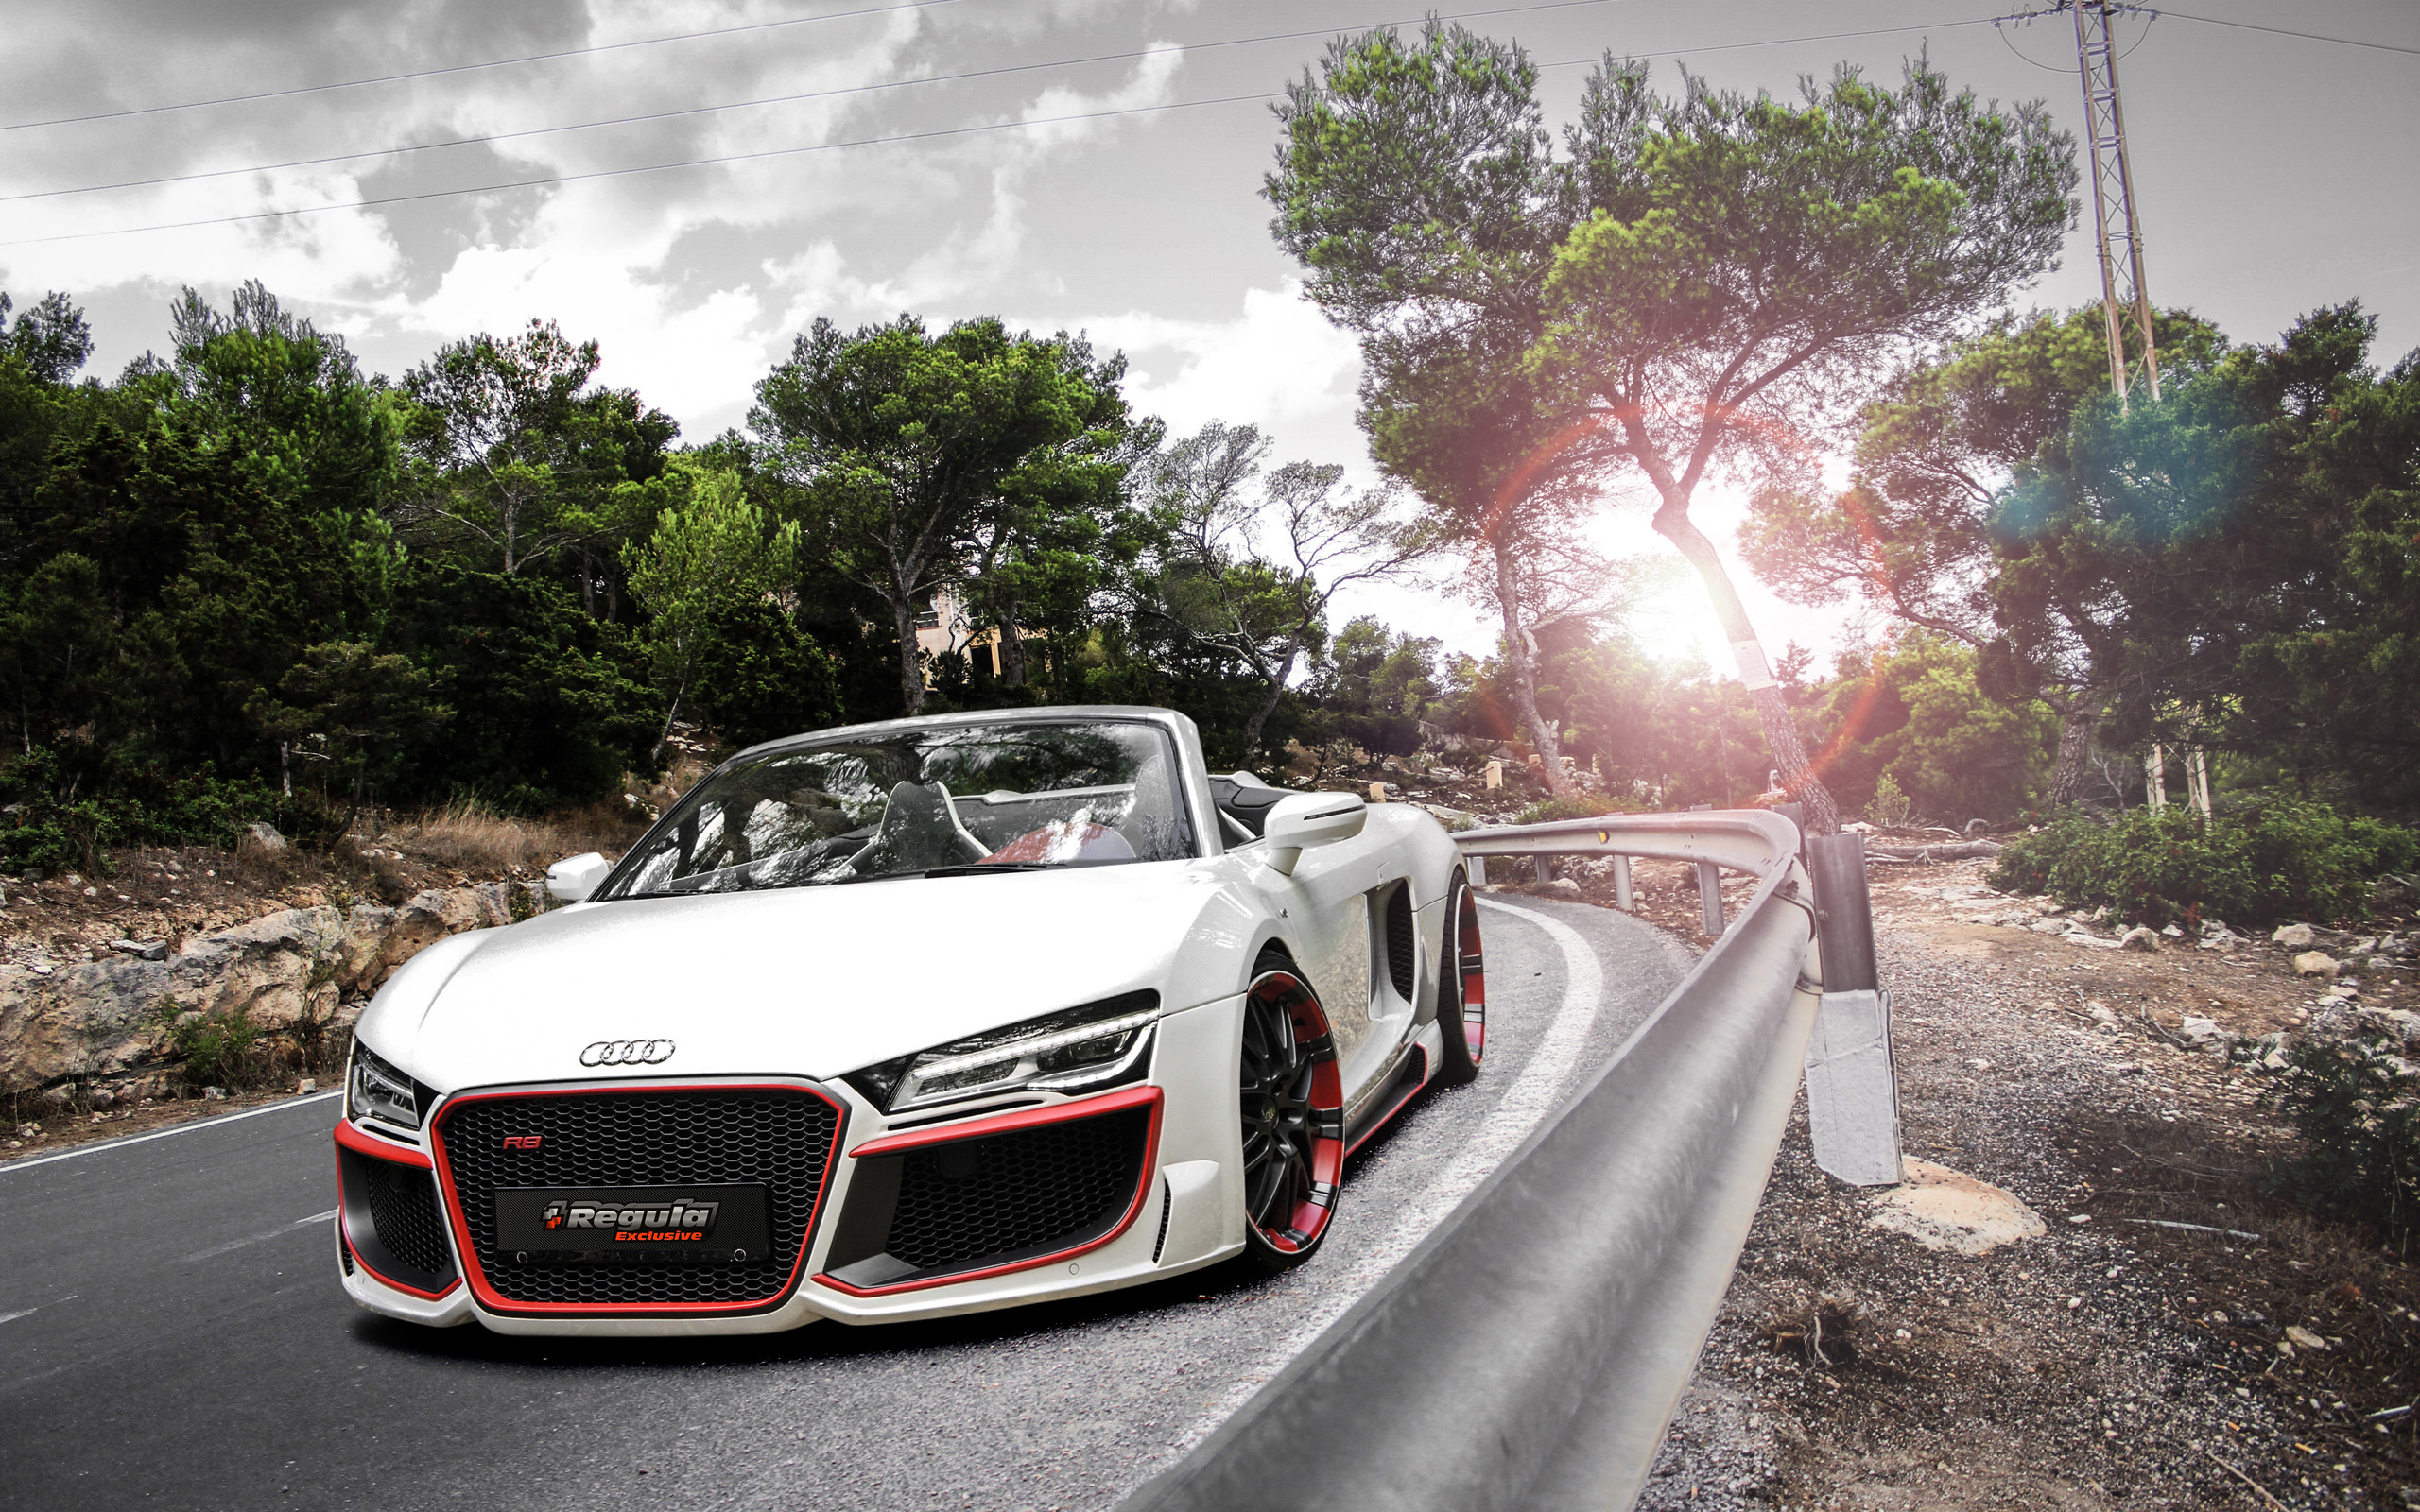
\includegraphics[scale=0.5]{src/diagram/test}
	\caption{The class diagram of the \rpntree within the \gnanal}	
	\label{dia:RPN-classdiagram}
\end{figure}

\newsavebox\mybox
\begin{lrbox}{\mybox}
	
	\begin{tikzpicture}[scale=0.6, every node/.style={scale=0.6}]
		\node (Plus) at (0,0) [objDia] {
			\textbf{f1}:RPNFunctionSymbol
			\nodepart{second}arithmeticSymbol: PLUS
		};
		\node (Times1) at (-4, -2 ) [objDia] {
			\textbf{f2}:RPNFunctionSymbol
			\nodepart{second}arithmeticSymbol: TIMES	
		};
		\node (Times2) at (4, -2) [objDia] {
			\textbf{f3}:RPNFunctionSymbol
			\nodepart{second}arithmeticSymbol: TIMES	
		};
		\node (cons1) at (-6, -4) [objDia] {
			\textbf{c1}:RPNConstant
			\nodepart{second}value: 2
		};
		\node (var1) at (-2, -4)[objDia] {
			\textbf{v1}:RPNVariable
			\nodepart{second}varName: x
		};
		\node (cons2) at (2, -4) [objDia] {
			\textbf{c2}:RPNConstant
			\nodepart{second}value: 4
		};
		\node (var2) at (6, -4) [objDia] {
			\textbf{v2}:RPNVariable
			\nodepart{second}varName: y
		};
		\draw[thickarrow] (Plus.south)  -- ++(0,-0.4) -| (Times1.north) node [pos = 0.4, above, font=\footnotesize]{left};
		\draw[thickarrow] (Plus.south)  -- ++(0,-0.4) -| (Times2.north) node [pos = 0.4, above, font=\footnotesize]{right};
		\draw[thickarrow] (Times1.south)  -- ++(0,-0.5) -| (cons1.north) node [pos = 0.4, above, font=\footnotesize]{left};
		\draw[thickarrow] (Times1.south)  -- ++(0,-0.5) -| (var1.north) node [pos = 0.4, above, font=\footnotesize]{right};
		\draw[thickarrow] (Times2.south)  -- ++(0,-0.5) -| (cons2.north) node [pos = 0.4, above, font=\footnotesize]{left};
		\draw[thickarrow] (Times2.south)  -- ++(0,-0.5) -| (var2.north) node [pos = 0.4, above, font=\footnotesize]{right};
	\end{tikzpicture}
\end{lrbox}

\begin{figure}
	\begin{tikzpicture}[
			scale=0.6,
			every edge/.append style = { dashedarrow },
			every node/.append style = { stdNode} ]
		\node (L) {\begin{tabular}{cc} mathematical expression: \\ 2*x+4*y \end{tabular} };
		\node[below = of L] (M)  {\begin{tabular}{cc} reverse polish notation: \\ +*x2*y4 \end{tabular} };
		\node[right = of M] (R) {\usebox\mybox};
		\draw (L.south) edge (M.north);
		\draw (M.east) edge (R.west);
	\end{tikzpicture}
	\caption{An example of the representation of the term $2*(x+4)$ as a graph using the \rpntree of \autoref{sec:rpntree}}
	\label{ex:rpntree}
\end{figure}


\section{\tool{SMT}-Problem}
\label{sec:smt-problem}
Also we have to consider an \textit{Satisfiability Modulo Theorie}-Problem (\tool{SMT}-Problem, we have to solve to derive a \gna fulfilling all the criterias of \autoref{def:gna}. Since \tool{SMT}-Problem solving is a big research topic on it's own we only consider the very basic of \tool{SMT}-Solving necessary to understand how the program solves the problem. \newline
%TODO: write it more mathematically
Within this approach we use the so called \code{Basic Structures} defined within \aprove to add assertions to the \solver using the \smtfactory. An example of the structure of the assertions can be found in \autoref{ex:assertion-structure}. %MAYBE: Class-dia?

\begin{figure}[H]
	\begin{lstlisting}[escapechar = !]
		!$\underbrace{
			\underbrace{
				\underbrace{\underbrace{3}_{(1)}*\underbrace{x_1}_{(2)}}_{(3)} \quad \underbrace{+}_{(4)} \quad ...
			}_{(5)} 
			\qquad
			\underbrace{\le}_{(6)}
			\qquad
			\underbrace{3}_{(7)}
		}_{(8)}$!
	\end{lstlisting}
	\caption{An example to show the structure of an assertion used for the \solver}
	\label{ex:assertion-structure}
\end{figure}

Such an example assertion can be split into different parts: 
\begin{enumerate}
	\item[(1)] \code{PlainIntegerConstant}'s as coefficients
	\item[(2)] \code{PlainIntegerVariables}'s as variables the \solver should derive values for such that all assertions are satisfied
	\item[(3)] A coefficient multiplied with a variables is represented by an \code{PlainIntegerOperation} with \code{ArithmeticOperationType} \code{MUL}
	\item[(4)] An \code{ArithmeticOperationType} of type \code{ADD}
	\item[(5)] The left hand side is one big \code{PlainIntegerOperation} consisting of the addition(4) of the multiplication (3) of coefficient's (2) and variables (2).
	\item[(6)] The \code{IntegerRelationType} defining the assertion. We only use the \textit{EQ (equal)} or \textit{LE (less than or equal)} relations.
	\item[(7)] The right hand side is only \underline{one} \code{PlainIntegerConstant}
	\item[(8)] The whole line is a \code{PlainIntegerRelation}, which can be transformed into the \code{SMTExpressionFormat} the \solver uses.
\end{enumerate}

We use a solver within \aprove to create a bunch of assertions restricting the possible solution space. Since we operate in integer arithmetic and use linear equations we can restrict the solver to only use \textit{quantifier free linear integer arithmetic}. In order to solve the problem given by the assertions the solver tries to derive a model satisfying all of them or derive an unsatisfiable core. \cite{sat2016}\newline

\begin{example}
	Consider the following assertions that should hold:\newline
	\vspace{-1em}
	\begin{figure}[H]
		\centering
		\begin{tabular}{cccc}
			$x \le y$ &	$x  < 5 $ &	$ x+ y \le 20$ &$y \neq 10$ \\
		\end{tabular}
	\end{figure}
	\vspace{-1em}
	Then a possible model would be $m_1 = \{x=6, y=6\}$. An other model would be $m_2 = \{x=6, y=7\}$. If we change the third rule to $x+y\le 10$ there is no model to the problem and we would receive the unsatisfiable core $c= \{x \le y$ $x  < 5$ $x+ y \le 10 \}$.
\end{example}

Since for \autoref{def:gna} the existence of a model is the crucial information, the model which should be derived is arbitrary among the set of possible models.

Further knowledge about \tool{SMT}-Problem solving can be gathered from the lecture "Introduction to Satisfiability Checking" or the \tool{SMT-RAT} toolbox for Strategic and Parallel SMT Solving by Prof. Dr. Erika Ábrahám and her team at the \textit{RWTH Aachen University} \cite{corzilius2015smt}.
